\section{Discussion}
\label{section:p450/discussion}
The physical score performs nearly as well as the fitted score indicating that the model is not over-fit to the training set.
Figure \ref{figure:idsite_other} presents a comparison of both IDSite models (physical and fit) to a number of other methods for prediction of P450 sites of metabolism.
Though the data sets used are not identical they are similar and overlapping for some compounds.
At all sensitivities IDSite is clearly the best performing protocol, with the physical and fit model performing very nearly identically.

At 90\% sensitivity, the QSAR method included roughly 20\% false positives, and MetaSite included 40\% false positives.
At the same sensitivity IDSite has a \textapprox1\% false positives rate.
This represents a significant improvement in prediction accuracy that has the potential to have a large impact on drug development.

\subsection{Significance of Sampling Stages}
\label{subsection:p450/discussion/sampling_stages}
\begin{figure}[h!]
\centering
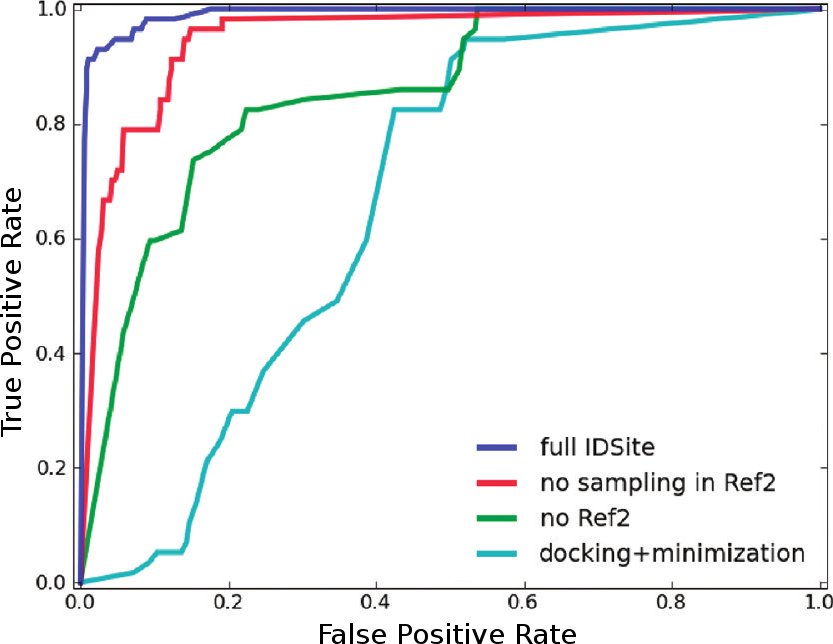
\includegraphics[width=0.5\textwidth]{figures/idsite/roc_sampling.png}
\caption{The effect of additional sampling on prediction of site of metabolism by P450.
The light blue series describes only performing the initial Glide docking stage followed by minimization.
The green series is obtained by using the set of structures obtained in the first minimization Monte Carlo sampling stage.
The red series is obtained by screening the structures obtained in the first sampling stage, and minimizing these structures using the constraints specified in Figures \ref{figure:second_sp2_constraints} and \ref{figure:second_sp3_constraints}.
The blue series makes use of the entire IDSite procedure.
The color scheme of these series corresponds to the colors of edges in Figure \ref{figure:idsite_overview}.}
\label{figure:idsite_roc_sampling}
\end{figure}

As shown in Figure \ref{figure:idsite_roc_sampling} at a given specificity, sensitivity increases with additional sampling.
For some compounds there are either no conformations predicted via the docking procedure where the site of metabolism is sufficiently close to the heme oxygen to react or the scoring metric used by the docking procedure prefers conformations which are far from the reactive site over more reactive conformations.
The sampling stages, and constraints are useful in guiding these initial docked poses into more active conformations.

The trajectory followed during the minimization Monte Carlo sampling stages differs appreciably for small and large ligands.
For smaller ligands, in many cases the poses after the first constrained minimization were among the lowest energy poses explored.
For about 40\% of these small ligands (24/56) the same predictions were obtained after the first minimization Monte Carlo sampling stage as after the full IDSite procedure.
However, for large ligands, the constraints and sampling continued to decrease the energy over the course of the sampling stages, indicating that especially for large compounds the second refinement stage is critical to obtaining accurate predictions.

\subsection{Induced Fit Effects}
\label{subsection:p450/discussion/induced_fit}
The catalytic site of cytochrome P450 is flexible, changing conformation to accommodate a large variety of different substrates \cite{li2004structural,scott2004structure}.
The Monte Carlo sampling stages reflect this flexibility allowing the substrate to settle into the active site, guided by harmonic constraints, and allows the side chains to alter their conformations to better accommodate and interact with the ligand.
Side chain dihedrals were found to change less for smaller ligands, illustrating that less rearrangement of the active site was necessary in order bind the substrate in an active conformation.
In larger ligands, some side chain dihedrals changed by larger amounts, especially for bulkier amino acids such as phenylalanine, with Phe120 and Phe483 changing by up to 40 and 60 degrees respectively for some ligands.

\subsection{Balancing Structural Contribution and Reactivity}
\label{subsection:p450/discussion/structure_effects}
As reflected in equation \ref{equation:curtin_hammett}, the binding energy and intrinsic reactivity are the determining factors in predicting sites of metabolism.
The IDSite procedure evaluates and uses both of these quantities in classifying possible sites of metabolism.
The combination of structural information and information about the intrinsic reactivity of a site allows IDSite to correctly predict cases which would not be possible using either of these methods alone.

One case of such a prediction is nortriptyline, since the two sites on the seven-membered aliphatic ring are difficult to distinguish only with their intrinsic reactivity, as they are almost equally reactive.
However, experiments show that only the (E)-10 site of nortriptyline is metabolized \cite{linnet1997metabolism}.
In IDSite, the poses with the (Z)-10 site close to the ferryl oxygen are all at least 10 kcal/mol higher in energy compared to the poses with the (E)-10 atom close to the ferryl oxygen. 
Such an energy gap is large enough for IDSite to correctly determine the (E)-isomer as the only metabolite. 
While structural effects are therefore clearly very important to determine nortriptylene's site of metabolism, the intrinsic reactivities also play a key role. 
This is again nicely illustrated with the example of nortriptyline, where a simply structure based method (without considering intrinsic reactivities) would predict the site of metabolism as being an aromatic hydroxylation due to the favorable energy of the corresponding poses.
Therefore, IDSite is able to correctly balance the subtle effects stemming from intrinsic reactivity and structural fit.

Another case which illustrates the importance of balancing reactivity and structural information is brofaromine.
Experiments show that the major site of metabolism by CYP2D6 is O-demethylation \cite{feifel1993role}.
The intrinsic reactivity of the site of metabolism (4.7 kcal/mol) is very close to those of sites on the aromatic rings (non-sites of metabolism, 3.3 to 4.9 kcal/mol).
Due to the receptor geometry, it is impossible for the atoms on the furan ring to get close to the ferryl oxygen while still attaining the salt bridge with either Glu216 or Asp301.
Therefore, no poses which which would have predicted reaction on the furan ring satisfied the geometric constraints and those sites were correctly predicted as sites of non-metabolism. 
Although poses which satisfied the geometric constraints and placed the benzene ring in the metabolic site, these poses are strongly disfavored energetically by more than 20 kcal/mol. 
This indicates that taking the interactions between the ligand and the receptor into account, IDSite is able to make the prediction of the site of metabolism for brofaromine in good agreement with the experimental observation.

% Methoxyphenamine is another case where the joint effects of intrinsic reactivity and the structural fit lead to the correct predictions.
% Methoxyphetamine is metabolized through O-demethylation and aromatic hydroxylation mediated by CYP2D6 \cite{geertsen1995metabolism}.
% These two sites not only have very close intrinsic reactivities (5.7 and 6.3 kcal/mol, Figure 20), but their lowest energy poses also have very similar energies. 
% The non-site of metabolisms are not selected by IDSite, either because of unfavorable intrinsic reactivity or because of high pose energies.
